\documentclass[sigconf,anonymous,10pt]{acmart}

\setlength{\textfloatsep}{10pt plus 2pt minus 2pt}
\setlength{\floatsep}{8pt plus 2pt minus 2pt}
\setlength{\intextsep}{10pt plus 2pt minus 2pt}
\setlength{\dbltextfloatsep}{10pt plus 2pt minus 2pt}
\setlength{\abovecaptionskip}{6pt}
\setlength{\belowcaptionskip}{0pt}

\usepackage{graphicx}
\usepackage{booktabs}
\let\Bbbk\relax
\usepackage{amsmath,amssymb}
\usepackage{subcaption}
\usepackage{tikz}
\usepackage{soul}
\definecolor{newhl}{HTML}{FFD9A3}
\newcommand{\hlnew}[1]{{\sethlcolor{newhl}\hl{#1}}}

\usetikzlibrary{arrows.meta, positioning}
\graphicspath{{figures/}}

\acmConference[AINTEC '26]{Proceedings of the 21st Asian Internet Engineering Conference}{December 1--3, 2026}{Taipei, Taiwan}
\acmYear{2026}
\copyrightyear{2026}
\acmArticleSeq{8}
\begin{document}

\title{The Local Path Not Taken: Traffic Tromboning and Routing Inefficiency in Pakistan}

\author{Anonymous Author(s)}
\affiliation{%
  \institution{Anonymous Institution}
}
\email{anonymous@example.com}

\renewcommand{\shortauthors}{Anonymous et al.}

\begin{abstract}
Despite being connected to multiple submarine and terrestrial Internet cables, Pakistan's Internet connectivity is far from ideal. With a concerted push towards online service delivery and economy digitization, the robustness of the local Internet connectivity becomes key. We use $15$ RIPE Atlas probes on the last-mile, connected to $9$ different ISPs in $7$ Pakistani cities in a week-long experiment, capturing $305,116$ ping and $200,292$ traceroute measurements. Measurements are made to $98$ websites that form a stratified proportional sample of the most popular content accessed from Pakistan across different sections of the critical infrastructure hosted by Pakistani operators, CDNs, and offshore operators.  

Across our sample, none of our $157{,}402$ traces to Pakistani-hosted and CDN-hosted sites crossed the peering fabric of either PKIX Lahore or PIE Karachi, despite dozens of ISPs holding physical connections there. The same gap shows up with content delivery networks: a handful of ISPs privately peer with major CDN operators while the rest do not, so identical CDN-hosted content can be up to $31$ times slower to reach depending purely on which ISP a user has. Path tromboning affects $5.5\%$ of accesses and is concentrated on a handful of destinations. Three sites account for $86\%$ of every tromboned trace we observe, and for each of them the split is by operator rather than by round: three of our nine ISPs reach the site domestically on essentially every attempt, and the other six never do. We recommend that both ISPs and CDN operators peer at Pakistan's IXPs, which would reduce domestic traffic tromboning and the CDN latency gap we measure.


\end{abstract}

\begin{CCSXML}
<ccs2012>
<concept>
<concept_id>10003033.10003079.10011704</concept_id>
<concept_desc>Networks~Network measurement</concept_desc>
<concept_significance>500</concept_significance>
</concept>
<concept>
<concept_id>10003033.10003083.10003090.10003091</concept_id>
<concept_desc>Networks~Topology analysis and generation</concept_desc>
<concept_significance>300</concept_significance>
</concept>
<concept>
<concept_id>10003033.10003039.10003045.10003046</concept_id>
<concept_desc>Networks~Routing protocols</concept_desc>
<concept_significance>100</concept_significance>
</concept>
</ccs2012>
\end{CCSXML}

\ccsdesc[500]{Networks~Network measurement}
\ccsdesc[300]{Networks~Topology analysis and generation}
\ccsdesc[100]{Networks~Routing protocols}

\keywords{Internet exchange points, traffic tromboning, CDN peering, Pakistan, developing regions, RIPE Atlas, network measurement, submarine cable resilience}
\acmArticleSeq{8}
\maketitle



\section{Introduction}
Pakistan has over $150$ million broadband internet users served mostly over seven cable systems~\mbox{\cite{pta2026telecom}}. Pakistan's Internet gets disrupted frequently by submarine cable faults. Since $2024$ alone, eight such faults have been reported~\cite{subtelforum2024pakistan, tribune2025aae1, aljazeera2025redsea, arabnews2025maintenance, pta2026smw5}.


Nearly $37$\% of the $200\text{k}$ most popular domains, ranked by global Tranco popularity, are either hosted by Pakistani network operators or, far more often, by international CDN operators, some of which maintain local caches inside Pakistani ISP networks ~\cite{tranco}. Reaching it quickly and resiliently to submarine cable faults, regardless of the user's ISP, requires the CDN or network hosting it to peer with every ISP, not just the best-connected one.
To achieve this for every ISP, not just the best connected one, local network and hosting providers must peer with each other.

Private peering solves this issue, but requires $O(n^2)$ peering sessions, where $n$ is the number of network and hosting providers. This puts a strain on the routers and the interconnection network. An Internet Exchange Point (IXP) provides a shared physical location where many operators can peer at once through a route server. CDN operators also prefer IXPs over private peering to place their caches~\cite{opalinski2024quest}. This results in reduced latency and packet loss to CDN-hosted content in addition to that hosted by local operators. 

There are four IXP sites across Pakistan, three sites under the umbrella of PKIX established in $2017$, and one named PIE powered by DE-CIX, established in $2024$. PKIX's members are exclusively ISPs and telecom operators, whereas PIE's membership also includes a couple of CDN operators.

PKIX claims that inter-ISP latencies routed internationally, previously at $100$ to $144$\,ms, drop to $1$ to $31$\,ms when routed through the exchange~\cite{pta2026}.
Despite this, IXP effectiveness in Pakistan is questionable, since it requires competing stakeholders' willingness to cooperate and connect their traffic.
Multiple studies have measured the extent of paths to local content tromboning through international transit providers in developing countries and found gaps in the effectiveness of IXPs~\cite{gupta2014, edmundson2016characterizing, obriain2017rebuilding}.    

To our knowledge, there is no recent study which measures the effectiveness of IXPs in Pakistan from a neutral vantage point.
To bridge this gap, we use active measurements from $15$ RIPE Atlas probes distributed across various Pakistani ISPs to measure the effectiveness of the IXPs. We run traceroutes and pings over a week-long window to $98$ websites spanning government, education, banking, news, and other sectors.
Using this dataset, we answer the following four research questions:

\begin{description}
  \item[RQ1] Does traffic to domestically hosted and CDN-hosted content in Pakistan cross the country's Internet eXchange Points?
  \item[RQ2] Do users of different ISPs in the same city get similar latency to domestically hosted and CDN-hosted content? 
  \item[RQ3] To what extent does Pakistani traffic to domestically hosted destinations trombone through foreign networks, which ISPs and transit paths are responsible, and what is the RTT cost?
  \item[RQ4] For destinations that trombone, does a local path demonstrably exist?
\end{description}

Our findings show that the IXPs are unused. For the destinations that account for most of the tromboning we observe, a domestic path exists but only for some operators: three of our nine ISPs reach them without leaving the country on essentially every round, and six never do. We also find that the resulting excessive latency penalty is unevenly distributed across ISPs. A particular ISP, for example, reaches Cloudflare hosted sites in roughly $2$ to $3$\,ms, while six others sit between $91$ and $130$\,ms to the exact same sites. Furthermore, $5.5\%$ of the requests in our dataset to websites hosted in Pakistan trombone. Where the same site is also reached domestically by other vantage points, avoiding the detour would cut RTT by about $56\%$ for the affected users, a median saving of roughly $75$ ms.

\section{Related Work}
\label{sec:related-work}
The value of local peering in mature markets is well established and framed primarily as latency optimisation: IXP paths for Italian ISPs are both faster and more stable than upstream transit, avoiding a detour through an intermediate network abroad~\cite{dibartolomeo2015}, and large exchanges such as DE-CIX and AMS-IX carry a substantial share of European and Asian interdomain traffic~\cite{ager2012, chatzis2013}. We adopt the Italian study's vantage-point design, national probes measuring national targets, but replace its hand-picked target list with a reproducibly sampled pool (\S\ref{subsec:sites}). In the developing world the same infrastructure often fails to deliver that benefit. Two thirds of African interdomain paths between residential networks and local Google caches detour through Europe before returning to a destination that was never far away~\cite{gupta2014}; correcting this would compress intra-continental latency to roughly 30~ms, echoing PKIX's own published figures of $1$ to $31$~ms through the exchange against $100$ to $144$~ms for the international alternative~\cite{pta2026}. Peering alone cannot fix tromboning where the content is not domestically hosted: more than half of Brazil's and Kenya's most popular domestic websites resolve to servers in the United States or United Kingdom, and roughly $13$\% and $50$\% of measured paths respectively trombone as a direct consequence~\cite{edmundson2016characterizing}, which is why we measure CDN-hosted as well as locally hosted sites. The same asymmetry appears in government hosting, where $68$\% of North American government sites but only $5$\% of South Asian ones are delivered from third-party infrastructure~\cite{kumar2024choices}. Underuse is not fixed destiny: Uganda's national exchange pushed peak traffic from roughly $300$~Mb/s to over $2$~Gb/s within a single year after a switching-fabric upgrade and the onboarding of Akamai's CDN~\cite{obriain2017rebuilding}.

Pakistan's international connectivity is concentrated almost entirely at a small number of Karachi landing stations operated by the same limited set of gateway licensees, while cross-border terrestrial alternatives remain commercially unused for reasons of state security policy rather than engineering cost~\cite{opalinski2024quest}. Three operators, ISP F, ISP H, and more recently ISP A, hold the only licensed international gateways, and every other domestic ISP buys upstream connectivity from one of them~\cite{pacra2026telecom}. Whether that concentration is why these ISPs have little incentive to peer with one another is a claim our routing data alone cannot test, but it is consistent with the pricing record: ISP F's partial $2006$ privatisation did not produce a decline in wholesale gateway pricing, unlike the mobile sector in the same country~\cite{gonzalez2026peering}. The closest prior Pakistan-focused measurement work found that Pakistan's traffic to its own South Asian neighbours, India, Bangladesh, and Bhutan among them, routes through Europe or Singapore rather than directly~\cite{ali2017internet}. That is the same detour pathology we study, but observed from within the country, with per-ISP and per-hop attribution rather than an aggregate ping benchmark. No prior work has tested whether the same failure occurs domestically inside Pakistan, or whether Pakistan's own exchanges are used once traffic never needs to leave the country.

\section{Methodology}
\label{sec:methodology}
Our measurement framework evaluates path selection, latency, and routing anomalies for Pakistani web infrastructure through active measurements conducted from diverse vantage points to a stratified random sample of popular websites. 
Below, we detail our target site selection, vantage point selection, and measurement protocols.

\subsection{Measurement Design}
\label{sec:measurement}
In a week long experiment, we measure ping latency and traceroutes to $98$ websites from 15 RIPE Atlas probes live in Pakistan at the time of the experiment, spanning $9$ ISPs across $7$ cities (Figure~\ref{fig:probe-map}). Due to ICMP filtering and throttling, one of these probe returned no usable traceroutes and contributes to the latency analysis only (\S\ref{sec:cleaning}). Several ISPs are covered by more than one vantage point, enabling within-ISP comparisons across locations.

Against each of the $98$ sites, we run two complementary measurements from all the probes: a traceroute every hour and a ping every thirty minutes.
We use Paris-style traceroute to TCP port~$80$ rather than ICMP for traceroute to reduce the effect of ICMP filtering and throttling.

In the following, we use bold-face to denote vector quantities, and regular font for scalars. Every ping measurement consists of three ICMP packets, so the ping measurement at time $t$ from probe $p$ to site $s$ results in a vector of RTT measurements: $\textbf{r}_{p, s, t} = [r_{p, s, t}^0, r_{p, s, t}^1, r_{p, s, t}^2]$, If any of the ICMP packets does not get a response, the corresponding RTT value is $NaN$. Similarly, each
traceroute measurement results in a vector $\textbf{h}_{p, s, t} = [\textbf{h}_{p, s, t}^0,
\textbf{h}_{p, s, t}^1, ..., \textbf{h}_{p, s, t}^{n_{p, s, t}}]$. Here $n_{p, s, t}$ is the
highest TTL value for which an ICMP packet was sent in that trace. Each $\textbf{h}_{p, s,
t}^i$ is itself a vector consisting of a hop IP address and the cumulative RTT value.
\subsection{Websites Selection}
\label{subsec:sites}

We curated a candidate pool of $1,814$ popular Pakistani websites, classified into critical-infrastructure sectors using the CISA taxonomy~\cite{cisa} and shown in Table~\ref{tab:cisa-sample}. The pool begins with every \texttt{pk} CC-TLD site in Tranco's top one million~\cite{tranco}. Because many popular Pakistani sites do not use that CC-TLD, we extended the set of popular sites on a per CISA sector basis. For financial services and healthcare, we hand-picked Pakistani entities from the top $100$ sites accessed from Pakistan according to Semrush~\cite{semrush}. For each of the remaining sectors, we used official lists published by the corresponding government regulators.

We resolved each site with \texttt{socket.gethostbyname()} and looked up the owning ASN through Team Cymru~\cite{cymru}. A site is \textit{Pakistani} if its IP resolves to a Pakistani ASN, \textit{CDN-hosted} if it resolves to a major content delivery network, and \textit{Abroad} otherwise.

Because IP geolocation is unreliable, we verify each inferred location against measured RTT: where a probe's ping beats the f-latency to the claimed coordinates, the geolocation must be wrong. This corrects the implied city for $34$ of the $40$ CDN-class sites without changing any site's class, and is consistent with Gharaibeh et al.~\cite{gharaibeh:imc:2011}, who find geolocation accuracy degrades sharply below the country level. The resulting corrections are reported with the rest of the cleaning in \S\ref{sec:cleaning}.

We drew $100$ sites by proportional stratified random sampling with seed $42$ for reproducibility, each CISA sector forming a stratum. Sector sizes are heavily skewed, so we floor each stratum at two sites. Within each stratum, we picked Pakistani, CDN, and Abroad sites in a $2:2:1$ proportion.

Hosting is heavily concentrated among a few operators. Cloudflare alone fronts $33$ of the $40$ CDN-hosted sites. The Pakistani class is led by ISP F ($5$ sites), followed by the Higher Education Commission (HEC) ($4$) with a long tail of $12$ single-site hosts. The $20$ Abroad sites are spread across $14$ providers at one to four sites each.

\begin{table}[t]
\caption{Candidate pool and sampled sites by CISA sector.}
\label{tab:cisa-sample}
\footnotesize
\begin{tabular*}{\columnwidth}{@{\extracolsep{\fill}}lrrrrr}
\toprule
\textbf{CISA Sector} & \textbf{Pool} & \textbf{Sampled} & \textbf{PK} & \textbf{CDN} & \textbf{Abroad} \\
\midrule
Commercial Facilities             & 1{,}236 & 58 & 22 & 24 & 12 \\
Govt.\ Services \& Facilities     & 182     & 11 &  4 &  5 &  2 \\
Education                         & 177     & 10 &  4 &  4 &  2 \\
Communications                    & 138     &  7 &  3 &  3 &  1 \\
Financial Services                &  42     &  4 &  2 &  1 &  1 \\
Energy                            &  11     &  3 &  1 &  1 &  1 \\
Healthcare \& Public Health       &  18     &  3 &  1 &  1 &  1 \\
Transportation Systems            &  10     &  2 &  1 &  1 &  0 \\
\midrule
\textbf{Total}                    & \textbf{1{,}814} & \textbf{98} & \textbf{38} & \textbf{40} & \textbf{20} \\
\bottomrule
\end{tabular*}%
\end{table}


\begin{figure}[t]
  \centering
  
\includegraphics[width=\columnwidth]{fig_probe_map.png}
  \caption{Vantage points by city. Bubble area is proportional to probe count.}
  \label{fig:probe-map}
\end{figure}

\begin{table}[t]
\caption{Probes by ISP and city.}
\label{tab:probes}
\footnotesize
\begin{tabular*}{\columnwidth}{@{\extracolsep{\fill}}lll}
\toprule
\textbf{ISP} & \textbf{Cities} & \textbf{Probes} \\
\midrule
A & Haripur, Karachi, Karachi & A1, A2, A3 \\
B & Islamabad                & B1 \\
C & Islamabad, Islamabad     & C1, C2 \\
D & Lahore                   & D1 \\
E & Faisalabad               & E1 \\
F & Karachi, Mianwali, Lahore$^*$ & F1, F2, F3$^*$ \\
G & Rawalpindi, Karachi      & G1, G2 \\
H & Lahore                   & H1 \\
I & Lahore                   & I1 \\
\midrule
\textbf{Total} & 9 ISPs, 7 cities & 15 probes \\
\bottomrule
\end{tabular*}
\smallskip
\raggedright
{\footnotesize $^*$F3 is kept only for ping analysis.}
\end{table}



\subsection{Data Cleaning}
\label{sec:cleaning}
A seven-day long ($11$–$18$ July 2026) experiment resulted in $218,480$ traceroute rows and $436,828$ ping records across the final 98-site sample from $15$ probes that were live at the time. One of these received no valid traceroute responses: we retain only its ping RTT for latency analysis, which means traceroute-based analysis draws on $14$ probes ($200,292$ rows) while ping-based analysis draws on 15 ($305,116$ rows).

The classification of sites as Pakistani, CDN and Abroad was done from a single vantage point before the experiment began. During the experiment, two sites initially labelled Pakistani, \texttt{toptop.net} and \texttt{youth.cn}, were found to sit behind a resolver-dependent load balancer. Every real ISP resolver returns their true Pakistani address, but our own centralised lookup landed on a foreign node that no real user reaches, so we removed both to avoid the discrepancy. A third site, \texttt{phf.gop.pk}, was also flagged during this check because a later re-resolution returned an unrelated United States address. Its traceroutes ran to a Pakistani address throughout, answering at a median of $22.1$\,ms from our probes, so it was retained. The final sample is $38$ Pakistani, $40$ CDN and $20$ Abroad sites, $98$ in total.

Any ping record $\mathbf{r}_{p, s, t}$ with $\min\limits_{i}(r_{p, s, t}^i)$ of $NaN$ is dropped from the dataset.
We also drop traceroute records where $n_{p, s, t}$ is $255$. If we do not receive a response from a hop in a traceroute record, or receive a response from a private IP address, or receive an RTT exceeding $500\,ms$, we consider it an invalid response. Such hops are excluded from all path-based statistics. These steps avoid noise due to ICMP-filtering and throttling which is common on the Internet. Finally, for tromboning analysis, we consider only records for probe-site pairs that have at least $50$ traceroute records for statistical significance.
\subsection{The Latency Ratio}
\label{sec:ratio}
To compare RTTs across probe-site pairs at very different distances, we normalise each measured RTT by the smallest one physics allows, following~\cite{bozkurt:dissecting:2018}. The result is dimensionless: a \emph{latency ratio} of $1$ means the path runs at its physical limit, and $k$ means it takes $k$ times longer.

For Pakistani and Abroad sites, which have a unique server IP address in our dataset, that floor is the f-latency, the round-trip time of straight fibre over the great-circle distance $d_{p,s}$ between probe $p$ and site $s$. We take $d_{p,s}$ from the Haversine formula~\cite{robusto:1957:cosine}, using probe coordinates from the RIPE Atlas API and server coordinates from IP geolocation, and assume $v_f = c/1.468 \approx 204{,}200$\,km/s, giving a ratio of $102\,r_{p,s,t}/d_{p,s}$ with $d$ in km. Probe-site pairs closer than $30$\,km (median RTT in our dataset of $5.6$\,ms) are excluded from the analysis, since the scaled result approaches $0$. .

CDN sites have no single server location, so the f-latency of \S\ref{sec:ratio} cannot be computed for them. Instead we ask what the best achievable RTT from probe $p$ would be. Probe $p$ can reach the site directly, as anycast routing sends it, or in principle over an overlay through another Pakistani probe $q$, paying the fibre cost from $p$ to $q$ and then reusing $q$'s access. We take whichever is better. Let $r_0(q,s) = \min_t r_{q,s,t}$ be the lowest RTT probe $q$ ever measured to site $s$, and let $d_{p,q}$ be the great-circle distance between probes $p$ and $q$, so that $d_{p,q}/102$ is the round-trip f-latency between them in milliseconds. The floor for probe $p$ is the smallest of these options over every candidate $q$,
\[
  \phi(p,s) \;=\; \min_{q}\left(\frac{d_{p,q}}{102} + r_0(q,s)\right),
\]
where $q$ ranges over all probes including $p$ itself, for which $d_{p,p} = 0$. The latency ratio of a CDN observation is $r_{p,s,t}/\phi(p,s)$. Including $q=p$ guarantees $\phi(p,s) \le r_0(p,s)$, so no observation can score below $1$, while the minimum over the other probes is what makes a poorly connected network score badly rather than perfectly.

   
\subsection{Tromboning Classification}
\label{sec:detector}

Paths to sites hosted abroad must exit Pakistan. Furthermore, if a CDN-hosted site is not replicated by the operator in Pakistan, the path to it would also need to exit Pakistan. Accordingly, we apply tromboning detection only to Pakistani-hosted sites.
Any IP addresses belonging to CDN operators appearing as intermediate hops on a Pakistani-hosted trace are treated like any other hop. 

To classify a trace as tromboned, we check the owning ASN of every intermediate hop in a traceroute to Pakistani sites in our cleaned dataset. If the owning ASN is a foreign entity, we classify it as tromboned with an exception. We found some IP addressed belonging to Shaw Communications (Canada), and Cogent Communications (US) in use inside Pakistan. We claim that they are in use inside Pakistan because they are reachable at an RTT that is impossible given their reported location. These IP addresses are excluded from our tromboning classification. 

There might still be false positives in our classifier due to inaccuracies in IP geolocation. To arrive at a more conservative classifier, we add one further condition. If the RTT reported by a hop that IP geolocation places outside Pakistan is below $40\,ms$, we do not classify the corresponding traceroute as tromboned.

The threshold is geometric rather than fitted to the traces it classifies. The furthest two points in Pakistan, Gwadar and the Khunjerab Pass, are separated by $1{,}801$\,km, which straight fibre traverses in $18\,ms$ round trip. Real domestic paths do not achieve that. Measuring latency per kilometre directly on our $192$ domestic probe--site pairs, the fastest runs at $1.30\times$ straight fibre, which places the ceiling for a domestic crossing of the country at roughly $23\,ms$. Pakistan's international connectivity is carried entirely by submarine cable, with the nearest foreign routers hundreds of kilometres beyond the Karachi landing stations, so a hop answering at $40\,ms$ or more cannot be domestic whatever its registration record says. The remaining margin absorbs router processing, queuing and last-mile access, and errs toward classifying a round as local. The threshold is never used to label a hop foreign on its own. It is only an additional check applied to a hop that IP geolocation has already placed outside the country.


\section{Results}
\label{sec:results}

Across the full week of measurement, ping packet loss averages $23.9\%$ overall, driven mainly by destination ICMP policy. Within the Pakistani hosted site class, the packet loss was $48.3\%$, versus $3.0\%$ for CDN sites, and $16.6\%$ for Abroad hosted sites. Median jitter is $7.45\,ms$, with probe F2 an outlier at $139.44\,ms$; that probe returned only $1{,}421$ traceroute rounds against roughly $6{,}200$ for the rest of the panel, so its variance reflects an intermittent connection rather than the paths it measured.


\subsection{IXP Crossing }
\label{sec:rq1}

Across the entire measurement week, not one of the $200,292$ traces we scanned crossed the peering fabric of PKIX Lahore or PIE Karachi, the two exchanges whose peering-LAN addressing we could verify. We could not obtain the peering-LAN addressing for PKIX Islamabad or PKIX Karachi and make no crossing claim for those two locations.

At PIE Karachi, ISP F and Tencent's ACE CDN both hold live, active route-server sessions, confirmed directly through the exchange's own real-time routing data. ISP F receives $650$ routes through this session, and ACE CDN announces into it. Yet in our own traceroutes, traffic from ISP F's probe destined to the sites hosted by ACE CDN uses a private link instead of PIE, bypassing a connection that demonstrably works.

ACE CDN and Zenlayer are the only major CDNs that participate at any Pakistani IXP. So peering at an IXP does not yet form a viable solution for an ISP as far as efficient access to CDN-hosted content is concerned.

\subsection{The CDN Cross-Section}
\label{sec:prelim-cdn}
We define three RTT cut-offs for CDN cache access: local ($<15\,ms$), regional ($15-50\,ms$), or far ($>50\,ms$).
Figure~\ref{fig:cdn_by_isp} shows the fraction of CDN-hosted site accesses, grouped by ISP, that reach a local, regional, or far cache.

Roughly $40\%$ of CDN-hosted content is reached at a regional cache regardless of ISP, but local access is rare: only three of the nine ISPs reach any content locally at all. The gap between the best and worst connected operators is large. Mean RTT to CDN content ranges from $20.3$\,ms for ISP C to $136.3$\,ms for ISP F, the largest operator in the panel, a difference of $116.0$\,ms or $85.1\%$. The best-connected ISP reaches $85\%$ of CDN content locally or regionally, with a median latency of $2.7\,ms$. In comparison, the six ISPs with no local access have median RTTs of $91-130\,ms$. Expressed with the latency ratio of \S\ref{sec:ratio}, the median cost of non-peering ranges from $1.5\times$ for the second-best network to $10.3\times$ for the worst, with the largest operator at $9.7\times$, and the worst quarter of ISP--site pairs exceeds $31\times$.


\begin{figure}[tb]
  \centering
  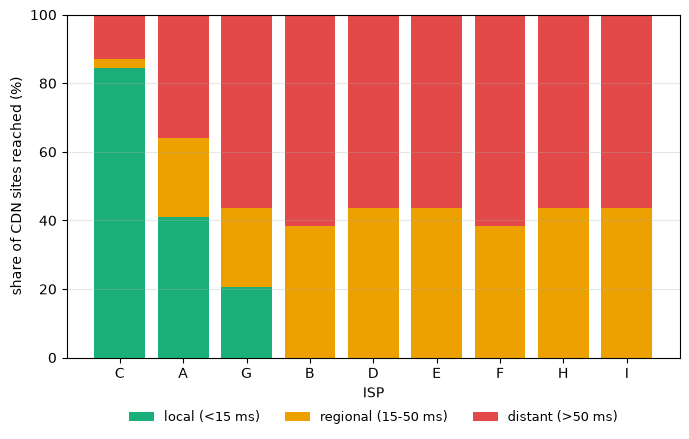
\includegraphics[width=\columnwidth]{figures/CDNaccessbyISP.png}
  \caption{CDN access by ISP}
  \label{fig:cdn_by_isp}
\end{figure}

\subsection{Same-City Latency Comparison}
\label{sec:rq2}

Users on different internet service providers within the same city do not necessarily experience similar latency to the same content, and whether they do depends heavily on what kind of content they are reaching. For domestic content, the gap is small. In Karachi, the same three internet service providers, ISPs A, G, and F, reach Pakistani-hosted sites at $18.4$, $20.3$, and $41.3$ ms median RTT, a $2.2\times$ spread. In Lahore, ISPs I, D, H, and C have RTTs between $17.5$ and $23.7$ ms, a $1.4\times$ spread.

However, CDN-hosted content is an entirely different matter. If the site is present at a cache within Pakistan, it is not too far from any of the probe locations being studied. Yet, we see pronounced differences in RTTs. In Karachi, ISP A has a median RTT of $4.4\,ms$ with $61.5\%$ requests served locally, while ISP G has a median RTT of $78.0\,ms$ with $41.0\%$ requests server locally, followed by ISP F at $129.8\,ms$ median RTT, with no request served from nearby cache. There is a 29.8$\times$ spread between the fastest and slowest ISPs operating in the exact same city. Lahore shows the same pattern: ISP C reaches a median RTT of of $2.8\,ms$ with $84.6\%$ of requests served locally, while ISPs D, H, and I cluster at $91$ to $95\,ms$ median RTT with zero local hits, a $34\times$ spread. For CDN sites, every ISP in a given city is equally close to a CDN's nearest cache, so any difference in performance between them is a peering choice, not a geography constraint. 

Since the local tier is an RTT threshold rather than ground truth, we cross-checked it for ISP C against Cloudflare's own edge, whose diagnostic endpoint (\texttt{/cdn-cgi/trace}) reports which point of presence answered each request. Querying it via Globalping from ISP C and five other Pakistani networks across all $33$ Cloudflare-hosted sites, $31$ of $33$ returned a Pakistani point of presence for ISP C, with TCP handshakes of 0 to $3$\,ms, physically impossible from outside the country. Two of those sites answered from Singapore for every other network tested, confirming ISP C alone reaches a genuinely local edge.



\subsection{Extent, Attribution, and Cost of Tromboning}
\label{sec:rq3}
If we use the presence of a foreign entity-owned IP address along a traceroute path as sign of tromboning, we find that $27.7\%$ requests in our dataset are affected by path tromboning. However, as discussed earlier, we found clear false positives in the form of Shaw Communications, and Cogent Communications IP addresses clearly being used inside Pakistan. If we exclude those, the overall tromboning rate drops to $7.3\%$. On the other hand, if we exclude the traces where the foreign-labeled hop has an RTT of at least $40\,ms$, the tromboning rate drops to $7.5\%$. If we apply both this minimum RTT threshold and the IP address false ownership filters, tromboning drops to $5.5\%$. We refer to this last figure as \textit{confirmed tromboning}.
Except for the naive classifier, these rates are notably lower than the 13\% reported by Edmundson et al.\ for Brazil, the 50\% for Kenya, and the 66.8\% measured by Gupta et al.\ for intra-African paths ~\cite{edmundson2016characterizing, gupta2014}. 

We also found that this tromboning rate differed by the vantage point than by the actual destination, as demonstrated by the breakdown of confirmed tromboning across operators (Figure~\ref{fig:panel-source}): ISP C and ISP H show zero confirmed tromboning throughout the week, ISP A sits at $2.6$\%, ISPs B, D, E, G, and I cluster tightly between $7.7$\% and $7.9$\%, and ISP F, the largest operator, reaches $10.2$\%, the highest in the panel. One might wonder why the tromboning differs across probes served by the same ISP. We found that these differences are due to randomness in ICMP throttling and filtering behavior. Sometimes ICMP packets from one probe operated by an ISP were throttled while those from another were not.   


We investigated if certain ISPs are responsible for more tromboning than others due to routing inefficiencies. To this end, we detected the ISP that owns the \textit{domestic hanoff}, i.e., the last non-private IP address preceding the foreign IP address in a confirmed tromboned traceroute.
Out of $4{,}170$ confirmed tromboned traces, the domestic hand-off is attributable for $3{,}779$ of them ($90.6\%$). The remaining $391$ resolve no Pakistani autonomous system anywhere before the exit. They come from two vantage points, and in every case the foreign address appears at the seventh or eighth hop, so the earlier hops replied but were private addresses or unannounced backbone interfaces.

The attributable hand-offs are distributed among five providers. ISP H leads with $43.8\%$, followed by ISP F ($22.8\%$), ISP G ($12.1\%$), ISP A ($8.1\%$) and ISP E ($4.0\%$). The hand-off is frequently not the user's own network. Only $49\%$ of these traces leave the country on the network their probe belongs to, and ISPs B, D and I never reach the border on their own network at all, which is why ISP H carries the largest share while registering no tromboning of its own traffic. On the foreign side, $89.7\%$ of confirmed tromboned paths exit through a router in Equinix Singapore, $6\%$ through the United States and $4\%$ through Hong Kong, with the remainder scattered elsewhere.

By sector, tromboning is concentrated almost entirely in two categories: Financial Services at $58.3$\% and Government Services at $14.6$\%, with Commercial Facilities at $1.4$\% and every other sector at zero.

 \begin{figure}[t]\centering\includegraphics[width=\columnwidth]{figures/Trombone_rate.png}
   \caption{Tromboning rate per vantage (ISP and city) for PK-hosted sites only.}\label{fig:panel-source}\end{figure}

Local traces to Pakistani-hosted sites have a median minimum RTT of $25.1$\,ms against $118.0$\,ms for tromboned traces to the same class of site (Figure~\ref{fig:panel-cdf}). That comparison pools two different populations of sites rather than the same site under both conditions, so it is not a causal estimate. Only $7$ of the $13$ flapping pairs accumulate enough rounds in both states to be compared directly, which is too few to support one. For the four sites that are reached both locally and via a detour by different vantage points, a same-site comparison gives a smaller and more defensible figure. Weighting by the number of affected pairs, avoiding the detour would reduce RTT by $56\%$, a median saving of $75$\,ms. This rests on $12$ tromboning pairs across those four sites, since \texttt{ztbl.com.pk} and \texttt{fgeha.gov.pk} block ICMP entirely and cannot be measured this way.


The tromboning rate is stable over time. Hourly it ranges from $5.3\%$ to $5.9\%$ across the day, and daily it stays within $5.3$ to $5.8\%$ across all seven days, with no weekday to weekend difference.

\begin{figure}[t]\centering
\includegraphics[width=\columnwidth]{fig_local_vs_hairpin_cdf.pdf}
  \caption{CDF of min-of-$N$ RTT to Pakistani-hosted sites, local vs hairpinned traces.}\label{fig:panel-cdf}\end{figure}

\subsection{Existence of a Local Path}
\label{sec:rq4-localpath}
A domestic path demonstrably exists for the destinations that matter most, but only for some operators. The three sites that account for $86\%$ of all tromboned traces are each reached without leaving the country by ISP A on every one of its $168$ rounds per site, and by six of the nine operators on essentially none. This is a measurement rather than a blind spot: ISP A's Haripur probe resolves $3.96$ responding mid-path hops per trace, as many as the probes that do register tromboning. ISP C and ISP H also record no tromboning to these sites, but their probes resolve roughly one mid-path hop and none at all respectively, so for those two we cannot distinguish a domestic path from an invisible one. The path exists; six operators do not have it.

We label one of these sites, a financial services site, Site Z, to make the mechanism concrete. ISP A reaches it in $5.4$\,ms over a domestic connection. Six of the nine operators reach the same server only by routing abroad first, through Oman for ISP F and through Singapore for ISP D and ISP I, arriving at median latencies $15$ to $33$ times slower. Every path that does leave the country enters the destination's network through the same ISP A edge, so the domestic path is not merely possible in principle but already carries the traffic of one operator.

At the level of individual probe--site pairs the picture is consistent. Of the $444$ valid pairs on Pakistani-hosted sites, $415$ never tromboned in any round, $16$ tromboned in every round, and $13$ tromboned in some rounds but not others. The unit here is the probe--site pair, meaning one vantage point reaching one site, so a site measured from twelve probes contributes twelve pairs. We do not treat the $13$ alternating pairs as independent evidence of an available domestic path. Requiring a confirmed AS-path change rather than a hop that stopped replying, only one of the thirteen qualifies.

Only $8$ of the $37$ Pakistani-hosted sites were ever confirmed tromboned from any vantage. The other $29$, $78\%$ of the total, stayed local all week, and none of the $8$ is tromboned on more than $90\%$ of its traceroutes. Tromboning under this standard is therefore not a general property of Pakistani hosting. It is concentrated in a small, identifiable minority of sites, consistent with the sector attribution of \S\ref{sec:rq3}, where Financial Services and Government Services account for nearly all of it.


\subsection{Latency Ratio by Site Type}
\label{sec:prelim-ratio}
Figure~\ref{fig:ratio-cdf} gives the latency ratio (\S\ref{sec:ratio}) as a CDF over $486$ unicast probe--site pairs. Of these, $192$ are Pakistani and $294$ are Abroad, and they are shown together with $546$ CDN pairs. Pakistani sites have a median of $2.98$$\times$ with a heavy tail. Around $26.6$\% exceed $10$$\times$, reaching as high as $75.17$$\times$, and this tail is spread across four ISPs rather than concentrated in one noisy vantage point.

That tail is largely an access-link artefact rather than a routing one. The clearest sign is that the worst ratios belong to the \emph{shortest} connections. The $23$ Pakistani pairs scoring above $15\times$ are located a median of $187$\,km apart, while the $123$ scoring below $5\times$ are $1{,}032$\,km apart, more than five times further. Their measured RTTs are almost the same, at $35.8$ vs $21.8$\,ms. What differs is the denominator. The ratio divides measured RTT by a floor derived from distance, so a close by pair has a tiny floor, and the same few milliseconds of fixed access overhead inflates its ratio far more than it does a pair that is far apart. The two flat stretches in the Pakistani curve, near $5\times$ and past $15\times$, are the boundaries between these distance groups in our vantage points rather than between good routes and bad ones.

Abroad pairs show the same reversal more starkly. Those scoring above $5\times$ are a median of $2{,}404$\,km apart, less than half the $5{,}444$\,km of those below. Their median RTT is lower, too, at $145.8$ vs $156.3$\,ms, even though their latency ratio is more than three times higher.

Subtracting each probe's own last-mile floor, meaning its fastest RTT to any Pakistani site, drops the Pakistani median on a three-day snapshot from $2.9$$\times$ to $1.9$$\times$. This is below the foreign figure of $2.4$$\times$. Nor is the remainder explained by geography. Distance explains most of the variation for Abroad sites ($R^2=0.48$) but almost none for Pakistani ones ($R^2=0.022$). As a result, a domestic site $1,000$\,km away is not reliably slower than one 100\,km away. The domestic \emph{route} is efficient once access overhead is removed. What is left is a routing choice, consistent with \S\ref{sec:rq1}.

The CDN curve is separate. An anycast site has no fixed distance, so its bimodal shape reflects which cache each ISP reaches.

\begin{figure}[t]
  \centering
  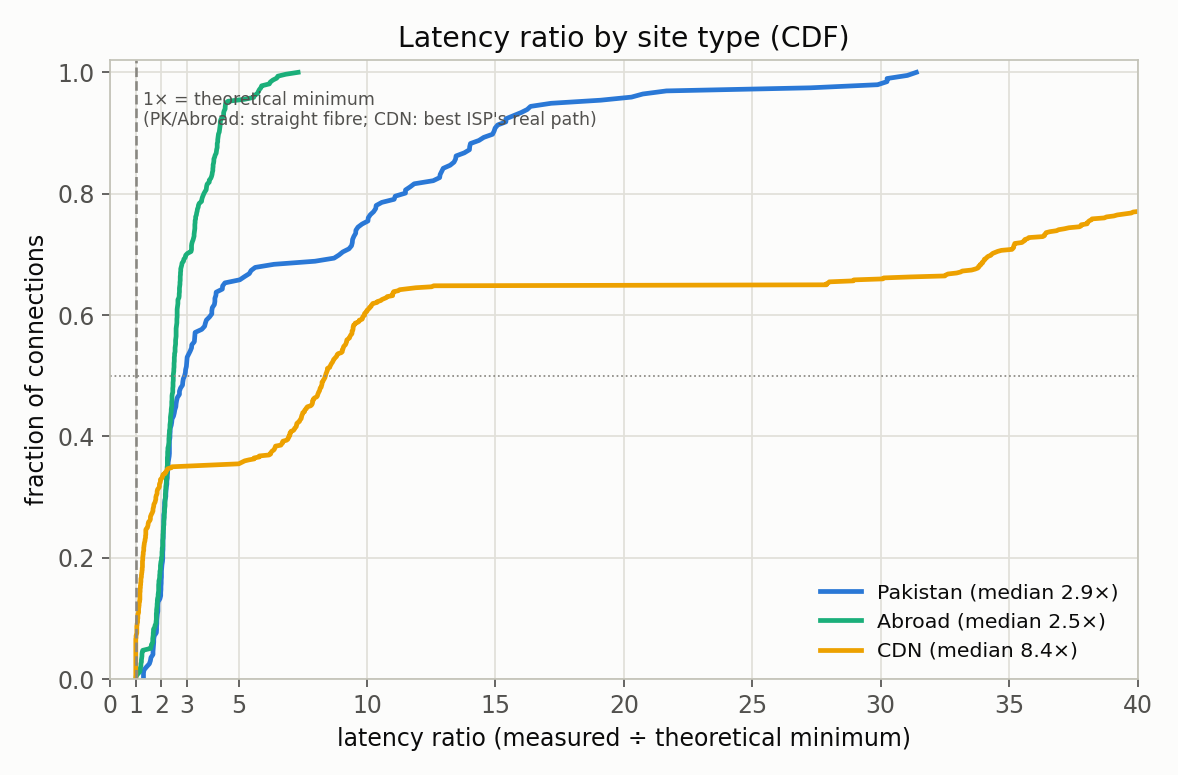
\includegraphics[width=\columnwidth]{ratio_cdf_all3.png}
  \caption{Latency ratio from all probes by site location.}
  \label{fig:ratio-cdf}
\end{figure}

Throughout, we report four indicators per probe--site pair, matching the metric set of prior IXP
measurement work~\cite{dibartolomeo2015}: minimum round-trip time (the primary latency measure,
\S\ref{sec:cleaning}); jitter, the standard deviation of round-trip time over all rounds for that
pair ($\sigma_{p,s,\bullet}$); ICMP ping packet loss, the fraction of ping packets that go
unanswered; and hop count, from the traceroute half.


\section{Discussion}
\label{sec:discussion}
A domestic path to Pakistani-hosted content can exist for one ISP and not for its competitors. Site Z (\S\ref{sec:rq4-localpath}) is reachable in $5$\,ms, proof that a fast path is technically possible. The problem is that the links which do get built are private and ad hoc, available only to whichever network happens to negotiate one, while every other ISP defaults to the international detour instead. The same asymmetry shows up in the CDN numbers. ISP F, the single largest operator, has the most to gain from better peering. If it matched ISP C's peering, its mean CDN RTT would fall by $116$\,ms, an $85.1$\% reduction, yet it is currently the worst-connected ISP in the panel.

That is consistent with the market-structure account raised earlier (\S\ref{sec:related-work}). An incumbent facing limited competitive pressure has little reason to invest in a connection its customers cannot easily punish it for skipping. An exchange changes that calculus. It turns a private negotiation each network has to justify on its own into a single, shared connection that every member reaches everyone else through, exactly the shift from present-but-not-exchanging to actively peering that we would expect.


That calculus is not hypothetical. Site Z shows it measured directly, one operator reaches it domestically while six detour abroad, so the cost of not peering is the gap between two paths that both exist today. The same best-achievable-RTT construction from \S\ref{sec:ratio} bounds the cost for the remaining tromboned pairs, which have no local round to compare against. Either way, the cost of not peering is not a rounding error.


Three limitations bound these claims. First, our vantages are fixed-broadband RIPE Atlas probes, while most of Pakistan's $150$ million users connect over mobile networks we have no vantage on; mobile-core routing may differ.
Second, RIPE Atlas measures latency and paths, not traffic volume, so we quantify tromboning's per-path cost, not its aggregate economic cost in purchased transit and foreign exchange; a traffic-weighted estimate is future work. Third, a low traceroute RTT to a CDN edge shows the network edge is local, not that the content is served locally; we do not treat one as proof of the other. 

\section{Conclusion}
Pakistan's exchanges already have dozens of connected members, including live, working sessions between ISP F and a few CDN operators, yet not one of $200,292$ traces crossed either exchange we could verify over a full week of measurement. We recommend that domestic ISPs and CDN operators peer actively at these exchanges, following Uganda's precedent, whose national IXP saw traffic grow six-fold within a year of onboarding Akamai's CDN~\cite{obriain2017rebuilding}. For the ISPs already connected this is a matter of using a connection that already exists; for the operators still absent, Cloudflare, Akamai, Google, and Amazon among them, it means joining the exchange as other developing regions already have. Leaving this unresolved keeps the country more exposed than it needs to be the next time a submarine cable fails.
\bibliographystyle{ACM-Reference-Format}
\bibliography{references}


\end{document}
